\chapter{\label{ch:energyloss}Electromagnetic Energy Loss in Liquid Argon} 

%%%%%%%%%%%%%%%%%%%%%%%%%%%%%%%%%%%%%%%%%%%%%%%%%%%%%%%%%%%%%%%%%%%%%%%%%%%%%%%%
% From COS
% This chapter will cover in more detail both the theory and measurement of
% electromagnetic energy loss in liquid argon. Energy loss for both electrons and
% photons will be discussed and the implications of this for electron
% reconstruction at different energy scales will be highlighted. 
% 
% The work in this section is complete and part of this work was reported in the
% document submitted for transfer of status.
%%%%%%%%%%%%%%%%%%%%%%%%%%%%%%%%%%%%%%%%%%%%%%%%%%%%%%%%%%%%%%%%%%%%%%%%%%%%%%%%

\minitoc

The energy loss of particles in liquid argon has important implications for the
reconstruction of different particles in a LArTPC, and will be relevant for the
analysis in Chapters \ref{ch:chargeid} and \ref{ch:michel} of  this thesis. This
chapter will cover in more detail the theory of electromagnetic energy loss in
liquid argon, highlighting the important features of the energy loss for 
muons, electrons, and photons.

In this chapter Section \mccorect{TODO.}

\section{Electromagnetic Energy Loss in Matter}
In matter, charged particles lose energy through a number of small successive
collisions with the electrons in the material, and by radiative processes which
produce additional particles in the material. The relative importance of the
collision and radiative stopping power depends on the mass and the energy of the
particle. For most particles, which are heavy compared to the electron, 
radiative energy losses are not important until very high energies, e.g. for a 
muon they are not important until momenta of around 100 GeV. However, 
radiative energy loss become important for electrons at tens of MeV 
\cite{PhysRevD.98.030001}. As a result, different theories are used to 
describe the energy loss of heavy particles and electrons in matter.

\subsection{Energy Loss for Heavy Charged Particles}
For heavy particles such as muons at moderate energies, the mean rate of 
energy loss per unit distance is described by the Bethe equation,
\begin{equation}
	- \left< \frac{dE}{dx}\right> = K z^2 \frac{Z}{A} \frac{1}{\beta^2} 
	\left[ \frac{1}{2} \ln \frac{2 m_e c^2 \beta^2 \gamma^2 W_{max}}{I^2} -
	\beta^2 - \frac{\delta(\beta \gamma)}{2}\right].
\end{equation}
The constants in this equation are detailed in reference
\cite{PhysRevD.98.030001}. $Z$ and $A$ are the atomic number and mass number of
the medium, $z$ is the charge of the scattering particle, $W_{max}$ is the 
maximum energy transfer per collision, $I$ is the average excitation energy, 
and $\delta$ is a density effect correction which is relevant in solids and 
liquids. 

Three important features of the energy loss in the Bethe formula are the minimum
ionising region, the relativistic rise, and the Bragg peak, these regions are
labelled in Figure \ref{fig:muon_dedx} which shows the $dE/dx$ for muons in 
argon as a function of momentum.
\begin{figure}

	\centering

	% TODO: make me nicer, and label me
	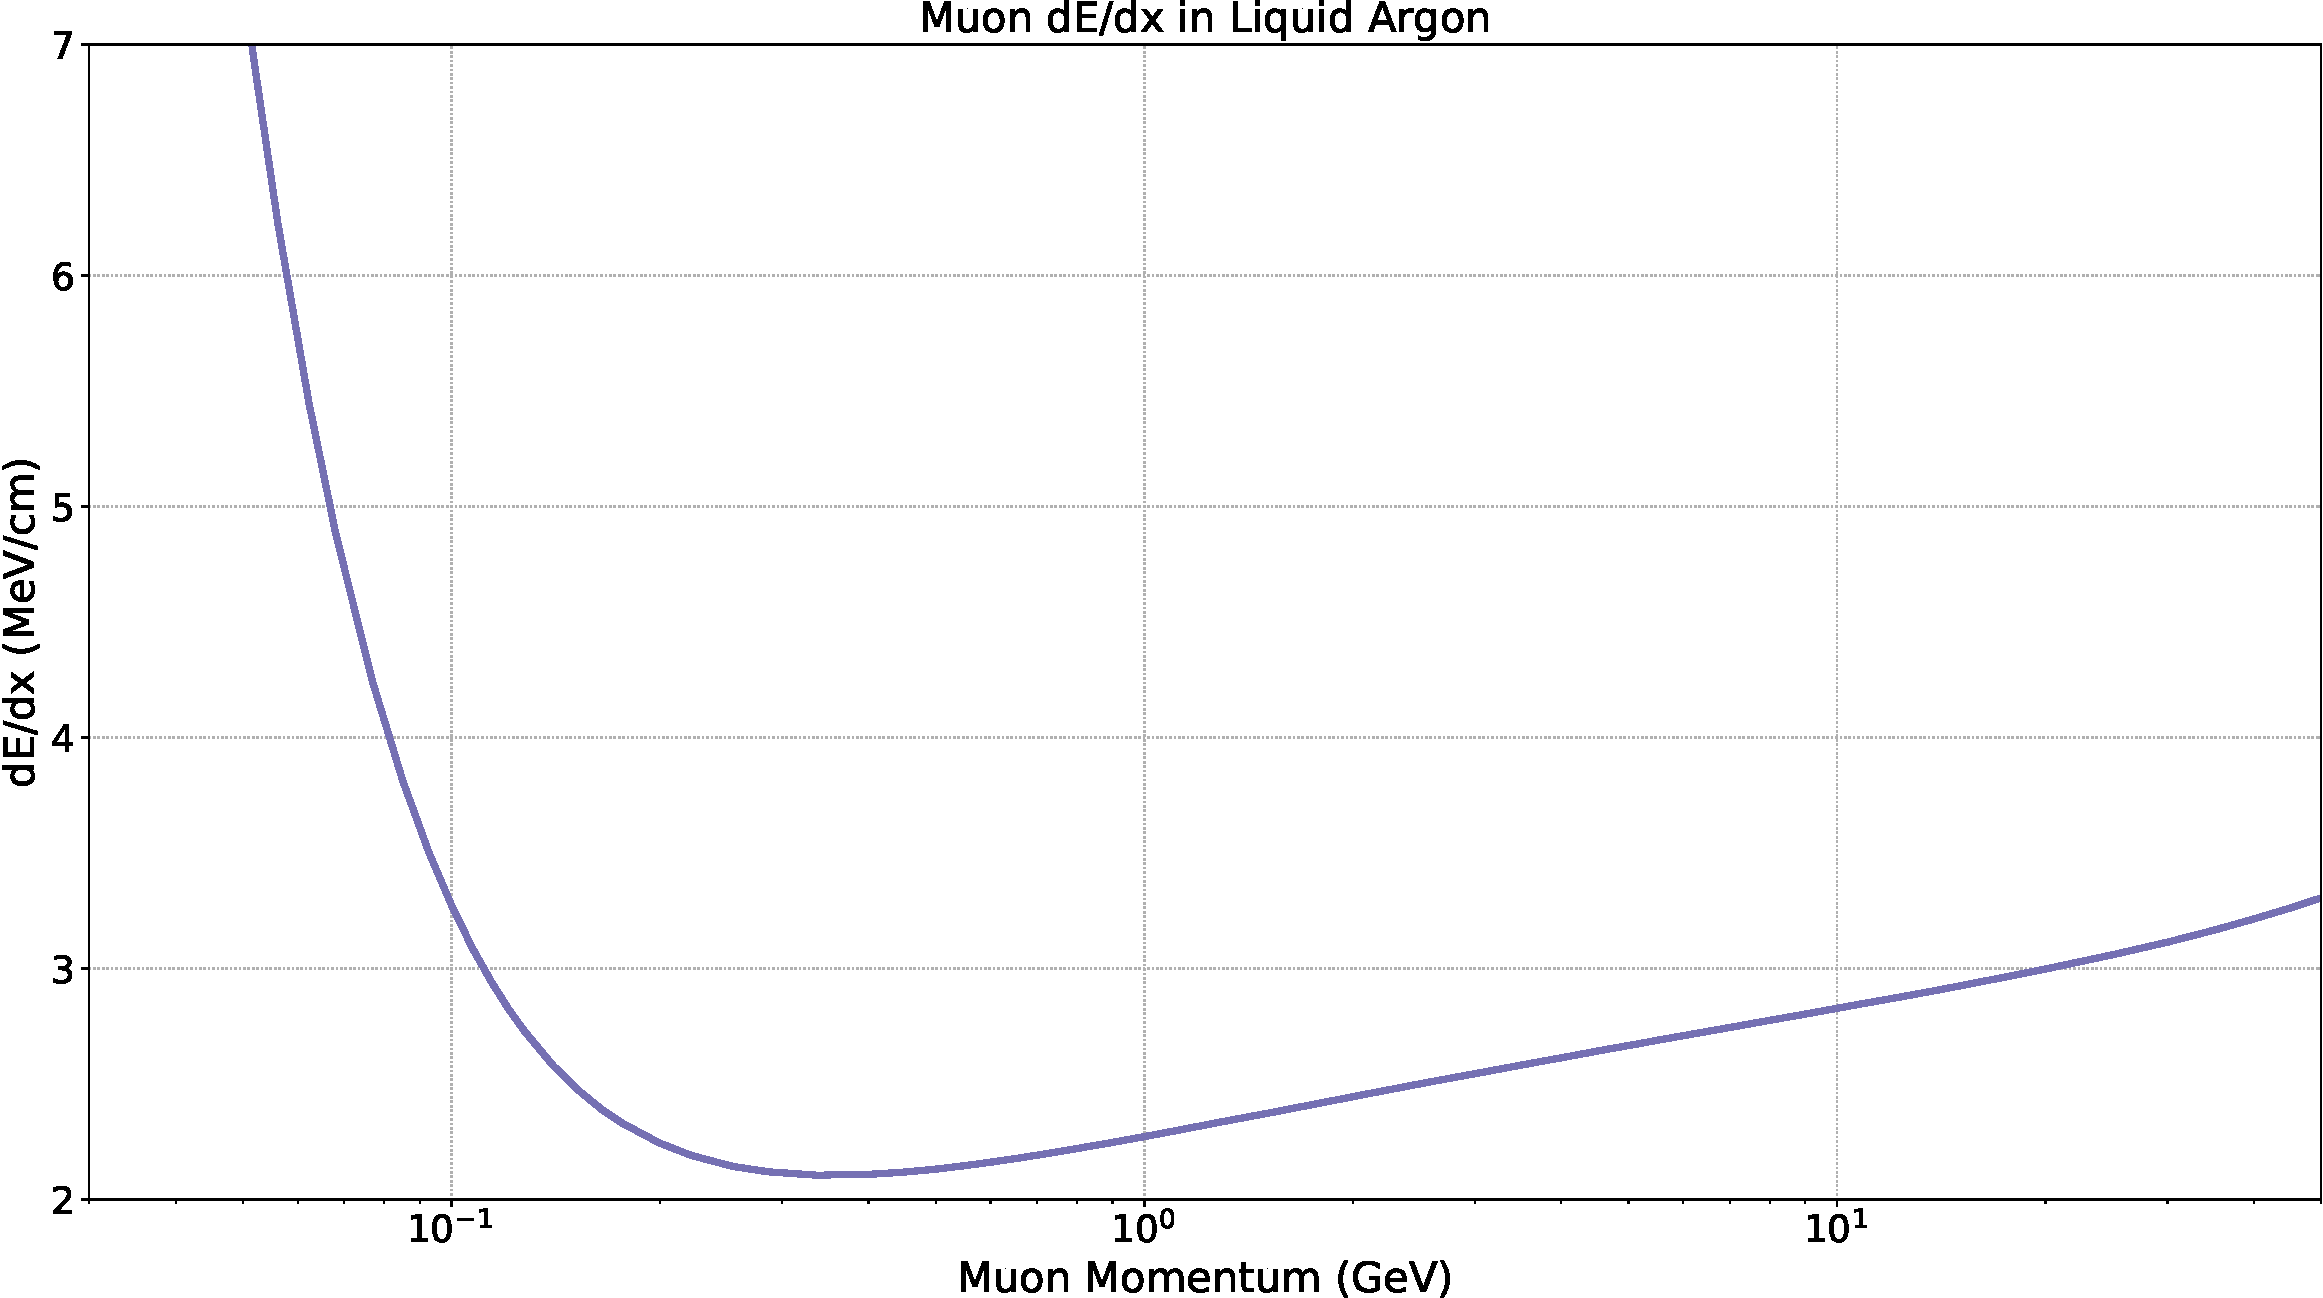
\includegraphics[width=\textwidth]{figures/muon_dedx_argon.pdf}

	\caption
	[Stopping power as a function of energy for muons in liquid argon.]
	{ Stopping power as a function of energy for muons in liquid argon. Data from
	\cite{pdg_atomictables}.}

	\label{fig:muon_dedx}

\end{figure}

\subsubsection*{Delta Rays}
Another feature of the electromagnetic energy loss of heavy particles that
impact reconstruction in LArTPCs is delta rays. Delta rays are energetic
electrons which are knocked out of their atoms when they collide with the heavy
particle, in liquid argon detectors these electrons are seen as small electron 
tracks which protrude from muon tracks. 

\subsection{Energy Loss for Electrons}
Electrons and positrons undergo different electromagnetic scattering processes
in matter, M{\o}ller scattering and Bhabha scattering respectively 
\cite{TODO}. These processes, which dominate electron and positron energy loss 
at low energies, have different cross sections which modify the energy loss in 
each case. At higher energies, radiative processes such as bremsstrahlung 
dominate. The two components of the electron stopping power are known as the 
collision stopping power and radiative stopping power.

\subsubsection*{Collision Stopping Power}
For electrons the collision stopping power is governed by M{\o}ller theory
which gives,
\begin{align}
	- \left< \frac{dE}{dx} \right> = \frac{1}{2} K \frac{Z}{A} \frac{1}{\beta^2}
	\bigg[ &\ln \frac{m_e c^2 \beta^2 \gamma^2 \left\{ m_e c^2 (\gamma - 1) / 2
	\right\} }{I^2} + (1 - \beta^2)  \\
	&- \frac{2\gamma - 1}{\gamma} + \frac{1}{8} 
	\left(\frac{\gamma - 1}{\gamma}\right)^2 - \delta \bigg]. 
\end{align}

\subsubsection*{Radiative Stopping Power}


\bigskip

The total electron stopping power in liquid argon is shown in Figure
\ref{fig:electron_dedx}, in addition to the collision and radiative components
which make up the total stopping power. The critical energy is often defined as
the energy at which the collision and radiative stopping power are equivalent,
for electrons and positrons in liquid argon the critical energy is around 32
MeV \cite{pdg_atomictables}.

\begin{figure}

	\centering

	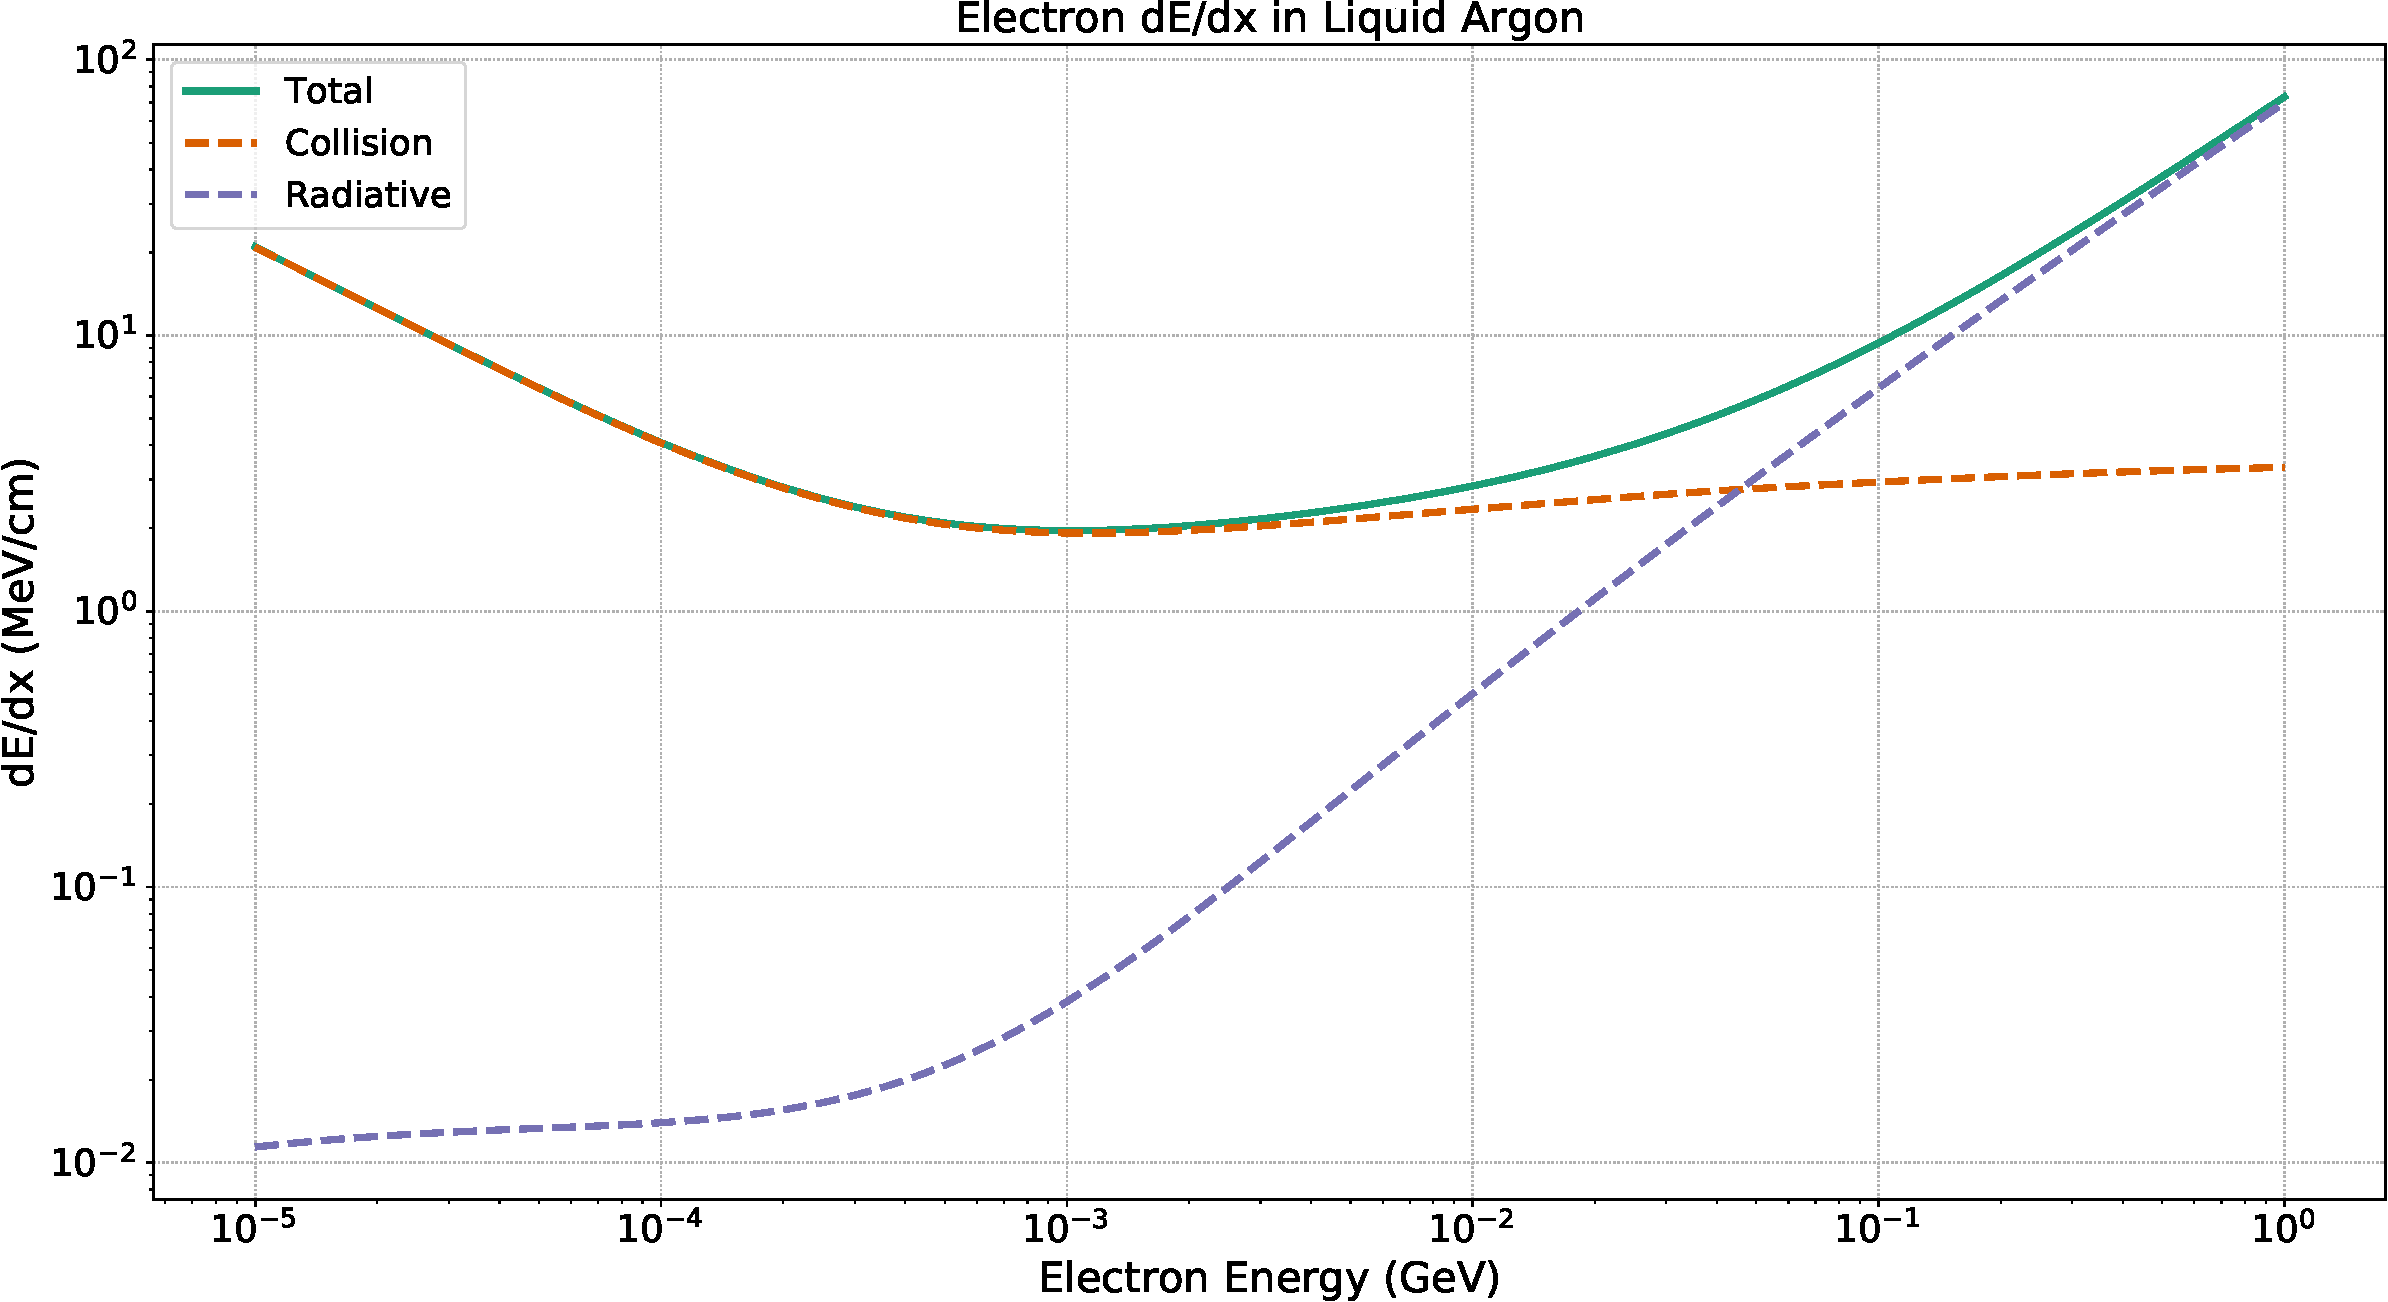
\includegraphics[width=\textwidth]{figures/electron_dedx_argon.pdf}

	\caption
	[Stopping power as a function of energy for electrons in liquid argon.]
	{ Stopping power as a function of energy for electrons in liquid argon. Data
		from \cite{estar}. }

	\label{fig:electron_dedx}

\end{figure}

\subsection{Energy Loss for Photons}

\section{Electron--Ion Recombination}
